\input{head.inc}

% Präambelbefehle für die Präsentation
\title[TET: Magnetostatik I - Grundlagen]{Magnetostatik I - Grundlagen}

\begin{document}
% 
% Frontmatter 
% 
%%%%%%%%%%%%%%%%%%%%%%%%%%%%%%%%%%%%%%%%%%%%%%%%%%%%%%%%%%%%%%%%%%%%%%%%%%%%%%%%%%%%%%%%%%%%%%%%%%%%%%%%%%%%%%%%%%%%%%%%%%%%% 

%% inserts the title page and the table of contents
\maketitle

% 
% Content 
% 
%%%%%%%%%%%%%%%%%%%%%%%%%%%%%%%%%%%%%%%%%%%%%%%%%%%%%%%%%%%%%%%%%%%%%%%%%%%%%%%%%%%%%%%%%%%%%%%%%%%%%%%%%%%%%%%%%%%%%%%%%%%%% 
\section{Magnetostatik I - Grundlagen}

\begin{frame}

  \frametitle{Ausgangspunkt Magnetostatik}

  \begin{itemize}[<+->]
  \item Die Magnetostatik betrachtet \alert{zeitunabhängige} magnetische Felder soweit diese durch \alert{Gleichströme} verursacht werden.
  \item Konstante magnetische Felder durch permanentmagnetische Stoffen spielen in der Regel keine Rolle.
    \item Wesentlicher Unterschied zur Elektrostatik ist, dass es \alert{keine magnetischen Monopole} gibt (jedenfalls keine, die nicht immer paarweise auftreten $\to$ \alert{Spineis}); führender Term ist also der Dipolterm.   
    \item Grundgleichungen:
	\begin{tabular}{cccc}
		
			allgemein	&	Elektrostatik	&	Stationäres Strömungsfeld	&	Magnetostatik\\
		\hline
			\(\rotation \HFeld[v] = \StromDichte[v] + \dfrac{\partial \DFeld[v]}{\partial t} \)
				&	
				&	 \(\left(\rotation \HFeld[v] = \StromDichte[v] \right)\)
				&	\(\boxed{\rotation \HFeld[v] = \StromDichte[v]} \)\\
				%\addlinespace
			\(\rotation \EFeld[v] = -\dfrac{\partial \BFeld[v]}{\partial t} \)
				&	\(\rotation \EFeld[v] = \vec{0} \)
				&	\(\rotation \EFeld[v] = \vec{0} \)
				&	\\
				%\addlinespace
			\(\divergenz \BFeld[v] = 0 \)
				&	
				&	
				&	\(\boxed{\divergenz \BFeld[v] = 0} \)\\
				%\addlinespace
			\(\divergenz \DFeld[v] = \laddichte{V} \)
				&	\(\divergenz \DFeld[v] = \laddichte{V} \)
				&	
				&	\\
				%\addlinespace
			\(\divergenz \StromDichte[v] + \dfrac{\partial \laddichte{V}}{\partial t} = 0 \)
				&	
				&	\(\divergenz \StromDichte[v] = 0 \)
				&	\(\left(\divergenz \StromDichte[v] = 0\right) \)\\
	\end{tabular}
\end{itemize}

\end{frame}


\begin{frame}

  \frametitle{Grundgleichungen der Magnetostatik}

  \begin{itemize}[<+->]
  \item Maxwell-Gleichungen:
    \begin{align*}
	& \text{differentielle Form}	&&	&&	\text{integrale Form}\notag \\
	& \rotation \HFeld[v] = \StromDichte[v]
		&& \rightarrow
		&& \oint\limits_{\rand(\Flaeche)} \HFeld[v](\Ortsr[v])\cdot \intweg[v] = \iint\limits_{\Flaeche} \StromDichte[v] \cdot \intflaeche[v] \\
	& \divergenz \BFeld[v] = 0
		&& \rightarrow
		&& \oiint\limits_{O(V)} \BFeld[v]\cdot \intflaeche[v] = 0
\end{align*}
\item Materialgleichung
\begin{equation*}
	\BFeld[v](\Ortsr[v]) = \mu_0 \text{M}_\mathrm{r}(\Ortsr[v], \HFeld[v], T, \dots)  \HFeld[v](\Ortsr[v]) \quad \to \quad \boxed{\BFeld[v](\Ortsr[v]) = \mu_0 \mu_\mathrm{r}  \HFeld[v](\Ortsr[v]) = \mu  \HFeld[v](\Ortsr[v])}
\end{equation*}
\item In der Elektrostatik folgte aus $\rotation \EFeld[v] = \vec{0}$, dass das elektrische Feld ein Gradientenfeld ist: $\EFeld[v] = -\gradient \SkalarPot$
\item Das ist in der Magnetostatik wegen \(\rotation \HFeld[v] = \StromDichte[v] \neq \vec{0} \) nicht der Fall.
  \item Aber: \(\divergenz \BFeld[v] = 0 \) $\to$ \(\BFeld[v] \) ist \alert{quellenfrei}


\end{itemize}
\end{frame}


\begin{frame}
  \frametitle{Das magnetische Vektorpotential}
  \begin{itemize}[<+->]
  \item Aus \(\divergenz \BFeld[v] = 0 \) und $\divergenz\rotation \vec{A} = 0$ folgt, dass $\BFeld[v]$ immer als \alert{Rotation eines Vektorfeldes} dargestellt werden kann. Siehe auch: \alert{Helmholtz-Theorem} bzw. \alert{Fundamentalsatz der Vektoranalysis}
  \item Dieses Feld $\VektorPot[v]$ ist das \alert{magnetische Vektorpotential}:
    $$
    \boxed{\BFeld[v] = \rotation \VektorPot[v]} \quad \left[ \VektorPot[v] \right] = \si{\volt\second\per\metre}
    $$
    \item Vorteil: $\divergenz \BFeld[v] = 0$ automatisch erfüllt
  \item lineares, isotropes Medium: \(\BFeld[v] = \mu(\Ortsr[v])\HFeld[v] \)
    $$
    \rotation \HFeld[v] = \rotation\left( \dfrac{1}{\mu(\Ortsr[v])}  \BFeld[v] \right) = \boxed{\rotation\left( \dfrac{1}{\mu(\Ortsr[v])} \rotation \VektorPot[v] \right) = \StromDichte[v](\Ortsr[v])}
    $$
    lineares, isotropes und homogenes Medium: \(\mu(\Ortsr[v]) = \mu \)
    $$
    \mu \rotation \HFeld[v] = \rotation \BFeld[v] = \rotation \, \rotation \VektorPot[v] = \boxed{\gradient\divergenz \VektorPot[v] - \laplace \VektorPot[v]= \mu \StromDichte[v](\Ortsr[v])}
    $$
  \end{itemize}
\end{frame}


\begin{frame}
  \frametitle{Eichtransformation}
  \begin{itemize}[<+->]
\item Wegen $\rotation\gradient\psi =\vec{0}$:
      $$
    \BFeld[v]' = \rotation \underbrace{\left(\VektorPot[v] + \gradient\psi\right)}_{\VektorPot[v]'} = \rotation \VektorPot[v] = \BFeld[v]  
    $$
  \item Das Vektorpotential ist bestimmt nur bis auf einen Summanden $\gradient\psi$.
  \item Anwendung auf $\rotation \, \rotation \VektorPot[v] = \mu \StromDichte[v]$:
    $$
    \rotation \, \rotation \VektorPot[v]' = \rotation \, \rotation \VektorPot[v] = \mu \StromDichte[v](\Ortsr[v])  
    $$
  \item Übergang $\VektorPot[v]' = \VektorPot[v] + \gradient\psi$: \alert{Eichtransformation} $\to$ $\BFeld[v]'=\BFeld[v]$ ist \alert{eichinvariant}
  \item Für die Divergenz gilt:
    $$
    \divergenz \VektorPot[v]' = \divergenz\left(\VektorPot[v] + \gradient\psi \right) = \divergenz\VektorPot[v] + \underbrace{\divergenz \gradient\psi}_{\ne 0}
    $$
    \item In $\boxed{\gradient\textcolor{red}{\divergenz \VektorPot[v]} - \laplace \VektorPot[v]= \mu \StromDichte[v](\Ortsr[v])}$ kann $\divergenz \VektorPot[v]$ \alert{beliebig} gewählt werden. 
  \end{itemize}
\end{frame}

\begin{frame}
  \frametitle{Coulomb-Eichung}
  \begin{itemize}[<+->]
  \item Für statische Probleme ist die \alert{Coulomb-Eichung} gut geeignet:
    $$
    \boxed{\divergenz\VektorPot[v] = 0} \quad \Longrightarrow \quad \boxed{\laplace \VektorPot[v]= -\mu \StromDichte[v](\Ortsr[v])}
    $$
  \item \alert{Achtung:} Der Laplace-Operator $\laplace$ für Vektorfelder muss im allgemeinen Fall (krummlinige Koordinaten) aus der Beziehung $\laplace \cdot = \gradient \, \divergenz \cdot - \rotation \, \rotation \cdot$ ausgerechnet werden.
  \item Hierbei \enquote{vermischen} sich die Komponenten wegen der Ortsabhängigkeit der Einheitsvektoren.
  \item \alert{Nur für kartesische Koordinaten} zerfällt die vektorielle Poissongleichung \enquote{einfach} in drei skalare Poissongleichungen:
    \begin{align*}
	& \laplace \VektorPot_\mathrm{x} = -\mu  \StromDichte_\mathrm{x}\\
	& \laplace \VektorPot_\mathrm{y} = -\mu  \StromDichte_\mathrm{y}\\
	& \laplace \VektorPot_\mathrm{z} = -\mu  \StromDichte_\mathrm{z} \text{ mit} \\
	& \VektorPot[v] = \VektorPot_\mathrm{x}  \einheitsvek{x} + \VektorPot_\mathrm{y}  \einheitsvek{y} + \VektorPot_\mathrm{z}  \einheitsvek{z}\\
	& \StromDichte[v] = \StromDichte_\mathrm{x}  \einheitsvek{x} + \StromDichte_\mathrm{y}  \einheitsvek{y} + \StromDichte_\mathrm{z}  \einheitsvek{z} \\
  &\laplace = \dfrac{\partial^2}{\partial x^2} + \dfrac{\partial^2}{\partial y^2} + \dfrac{\partial^2}{\partial z^2} \text{ (skalarer Laplace-Operator)}
\end{align*}

  \end{itemize}
\end{frame}


\begin{frame}
  \frametitle{Laplace-Operator in Zylinderkoordinaten}
  \begin{itemize}[<+->]
  \item Z.B. in Zylinderkoordinaten (\(\rho,\,\varphi,\,z \)) ergibt sich 
\begin{align*}
	\laplace \VektorPot_{\uprho} - \dfrac{2}{\rho^2} \dfrac{\partial \VektorPot_{\upvarphi}}{\partial \varphi} - \dfrac{\VektorPot_{\uprho}}{\rho^2} &= -\mu \StromDichte_{\uprho} \\
	\laplace \VektorPot_{\upvarphi} + \dfrac{2}{\rho^2}  \dfrac{\partial \VektorPot_{\uprho}}{\partial \varphi} - \dfrac{\VektorPot_{\upvarphi}}{\rho^2} &= -\mu \StromDichte_{\upvarphi} \\
	\laplace \VektorPot_\mathrm{z} &= -\mu  \StromDichte_\mathrm{z}
\end{align*}
mit
\begin{equation*}
	\laplace = \dfrac{1}{\rho} \dfrac{\partial}{\partial \rho} \rho \dfrac{\partial}{\partial \rho} + \dfrac{1}{\rho^2} \dfrac{\partial^2}{\partial \varphi^2} + \dfrac{\partial^2}{\partial z^2} \text{ (skalarer Laplace-Operator)}
\end{equation*}
  \end{itemize}
\end{frame}

\begin{frame}
  \frametitle{Lösung für das Vektorpotential}
  \begin{itemize}[<+->]
  \item Für den Fall \alert{kartesischer Koordinaten} ergeben sich drei Poisson-Gleichungen (offensichtlich nicht für Zylinderkoordinaten) $\to$ \alert{Lösungsmethoden anwendbar!}
    \item Analog zum Coulomb-Integral ergibt sich
\begin{align*}
	& \VektorPot_\mathrm{x}(\Ortsr[v]) = \dfrac{\mu}{4 \uppi} \iiint\limits_{\volumen} \dfrac{\StromDichte_\mathrm{x}(\Ortsr[vs]) }{\left| \Ortsr[v] - \Ortsr[vs] \right|} \intvolumen' \\
	& \VektorPot_\mathrm{y}(\Ortsr[v]) = \dfrac{\mu}{4 \uppi} \iiint\limits_{\volumen} \dfrac{\StromDichte_\mathrm{y}(\Ortsr[vs]) }{\left| \Ortsr[v] - \Ortsr[vs] \right|} \intvolumen' \\
	& \VektorPot_\mathrm{z}(\Ortsr[v]) = \dfrac{\mu}{4 \uppi} \iiint\limits_{\volumen} \dfrac{\StromDichte_\mathrm{z}(\Ortsr[vs]) }{\left| \Ortsr[v] - \Ortsr[vs] \right|} \intvolumen'
\end{align*}
\item Dies lässt sich wieder \alert{koordinatenfrei} schreiben:
\begin{equation*}
	\boxed{\VektorPot[v](\Ortsr[v]) = \dfrac{\mu}{4 \uppi} \iiint\limits_{\volumen} \dfrac{\StromDichte[v](\Ortsr[vs])}{\left| \Ortsr[v] - \Ortsr[vs] \right|} \intvolumen'} 
\end{equation*}
\item Für einen \alert{Stromfaden} folgt der Spezialfall
\begin{equation*}
	\VektorPot[v](\Ortsr[v]) = \dfrac{\mu}{4 \uppi} \oint \dfrac{\Strom}{\left| \Ortsr[v] - \Ortsr[vs] \right|} \intweg[vs] \text{ entlang des Stromfadens} 
      \end{equation*}
  \end{itemize}
\end{frame}

\begin{frame}
  \frametitle{Gesetz von Biot-Savart}
  \begin{itemize}[<+->]
  \item Mit $\BFeld[v]=\rotation \VektorPot[v]$ und $\VektorPot[v](\Ortsr[v]) = \dfrac{\mu}{4 \uppi} \iiint\limits_{\volumen} \dfrac{\StromDichte[v](\Ortsr[vs])}{\left| \Ortsr[v] - \Ortsr[vs] \right|} \intvolumen'$ folgt
    $
    	\BFeld[v](\Ortsr[v]) = \dfrac{\mu}{4 \uppi} \iiint\limits_{\volumen} \rotation_\mathrm{r} \dfrac{\StromDichte[v](\Ortsr[vs])}{\left| \Ortsr[v] - \Ortsr[vs] \right|} \intvolumen'
    $
\item Man berechnet
\begin{align*}
	\rotation_\mathrm{r} \dfrac{\StromDichte[v](\Ortsr[vs])}{\left| \Ortsr[v] - \Ortsr[vs] \right|} &= \dfrac{1}{\left| \Ortsr[v] - \Ortsr[vs] \right|}  \cancelto{0}{\rotation_\mathrm{r} \StromDichte[v](\Ortsr[vs])} - \StromDichte[v](\Ortsr[vs]) \times \gradient_\mathrm{r} \dfrac{1}{\left| \Ortsr[v] - \Ortsr[vs] \right|} \\
		&= -\StromDichte[v](\Ortsr[vs]) \times \gradient_\mathrm{r} \dfrac{1}{\left| \Ortsr[v] - \Ortsr[vs] \right|} = -\StromDichte[v](\Ortsr[vs]) \times \left( -\dfrac{\left( \Ortsr[v] - \Ortsr[vs] \right)}{\left| \Ortsr[v] - \Ortsr[vs] \right|^3} \right) = \StromDichte[v](\Ortsr[vs]) \times \dfrac{\Ortsr[v] - \Ortsr[vs]}{\left| \Ortsr[v] - \Ortsr[vs] \right|^3}
\end{align*}
\item Damit folgt das das allgemeine \alert{Biot-Savart-Gesetz}
\begin{equation*}
	\boxed{\BFeld[v](\Ortsr[v]) = \dfrac{\mu}{4  \uppi} \iiint\limits_{\volumen} \dfrac{\StromDichte[v](\Ortsr[vs]) \times \left( \Ortsr[v] - \Ortsr[vs] \right)}{\left| \Ortsr[v] - \Ortsr[vs] \right|^3} \intvolumen'}
\end{equation*}
\item Für Stromfäden folgt
\begin{equation*}
	\boxed{\BFeld[v](\Ortsr[v]) = -\dfrac{\mu}{4  \uppi}  \Strom  \oint\limits_{\rand} \dfrac{\left( \Ortsr[v] - \Ortsr[vs] \right) \times \upd \Weg[vs]}{\left| \Ortsr[v] - \Ortsr[vs] \right|^3}} \text{ und }
	\boxed{\VektorPot[v](\Ortsr[v]) = \dfrac{\mu}{4  \uppi}  \Strom  \oint\limits_{\rand} \dfrac{\upd \Weg[vs]}{\left| \Ortsr[v] - \Ortsr[vs] \right|}}
\end{equation*}
  \end{itemize}
\end{frame}

\begin{frame}
  \frametitle{Stetigkeitsbedingung an Grenzflächen}
  \begin{itemize}[<+->]
  \item Die Stetigkeitsbedingungen wurden im Teil \enquote{Verhalten am Grenzflächen} bereits allgemein hergeleitet.
  \item Es gilt (Normalenvektor von 1 nach 2):
    \begin{align*}
	\BFeld[v]_2\cdot \vec{n} - \BFeld[v]_1\cdot\vec{n} &= 0 \\
	\HFeld[v]_2\cdot \vec{t} - \HFeld[v]_1\cdot \vec{t} & = \StromDichte[v]_\mathrm{F}\cdot \vec{t}_2\\
	\tangentialvektor_2 & = \normalenvektor \times \tangentialvektor
\end{align*}
\item Hiermit folgt auch das \alert{Brechungsgesetz für $\vec{J}_{\text{F}} = \vec{0}$}

  \resizebox{.35\linewidth}{!}{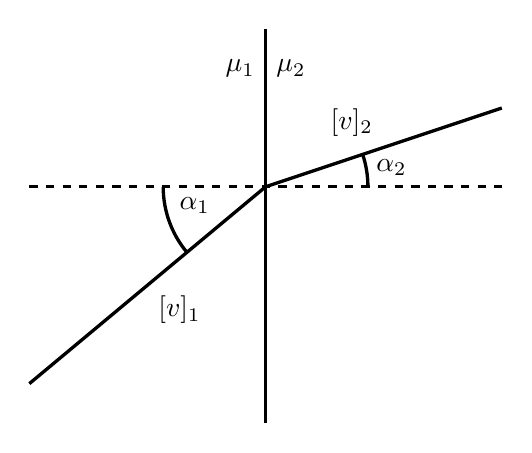
\begin{tikzpicture}[line width = 1.2pt, line join=round,x=1cm,y=1cm,>=stealth]
	% Grenzschicht
	\draw (0,-3) -- (0,2);
	% Referenznormale
	\draw [dashed] (-3,0) -- (3,0);
	% magnetischen Flussdichten
	\draw (-3,-2.5) -- (0,0);
	\draw ({-3/2},{-2.5/2}) node[anchor=north west] {$ \tetB[v]_1 $};
	\draw (0,0) -- (3,1);
	\draw ({3/2},{1/2}) node [anchor=south east] {$ \tetB[v]_2 $};
	% Winkel
	\draw (-1.3,0) arc (180:220:1.3);
	\draw (-0.9,0) node[anchor=north] {$ \alpha_1 $};
	\draw (1.3,0) arc (0:19:1.3);
	\draw (1.6,0) node[anchor=south] {$ \alpha_2 $};
	% Permeabilität
	\draw (0,1.5) node[anchor=east] {$ \mu_1 $};
	\draw (0,1.5) node[anchor=west] {$ \mu_2 $};
\end{tikzpicture}} \raisebox{1cm}{\boxed{\dfrac{\tan \alpha_1}{\tan \alpha_2} = \dfrac{\mu_1}{\mu_2}}}
  
  \end{itemize}
\end{frame}

\begin{frame}
  \frametitle{Energie im magnetostatischen Feld}
  \begin{itemize}[<+->]
    \item Analog zur Elektrostatik erhält man für die \alert{magnetische Energiedichte}
\begin{equation*}
	\boxed{\energiedichte_\mathrm{m} = \dfrac{1}{2} \cdot \HFeld[v] \cdot \BFeld[v]}
\end{equation*}
\item Für die gesamte \alert{magnetische Energie}
\begin{equation*}
	\boxed{\energie_\mathrm{m} = \dfrac{1}{2} \cdot \iiint\limits_{\volumen} \HFeld[v] \cdot \BFeld[v] \intvolumen} 
\end{equation*}
\item Ausdrücken mit Hilfe der elektrischen Stromdichte \(\StromDichte[v] \) (lineare, homogene und isotrope Medien): 
\begin{equation*}
	\energie_\mathrm{m} = \dfrac{1}{2 \mu} \cdot \iiint\limits_{\volumen} \BFeld[v]^2 \intvolumen
\end{equation*}
\item Weiter:
\begin{align*}
	\divergenz \left( \VektorPot[v] \times \BFeld[v] \right) &= \BFeld[v] \cdot \underbrace{\rotation \VektorPot[v]}_{\BFeld[v]} - \VektorPot[v] \cdot \underbrace{\rotation \BFeld[v]}_{\mu \StromDichte[v]} \\
		&= \BFeld[v]^2 - \mu  \VektorPot[v] \cdot \StromDichte[v]
\end{align*}
  \end{itemize}
\end{frame}

\begin{frame}
  \frametitle{Energie im magnetostatischen Feld (fortgesetzt)}
  \begin{itemize}[<+->]
\item Daraus:
\begin{align*}
	\energie_\mathrm{m} &= \dfrac{1}{2}  \iiint\limits_{\volumen} \VektorPot[v] \cdot \StromDichte[v] \intvolumen + \dfrac{1}{2 \mu} \cdot \iiint\limits_{\volumen} \divergenz \left( \VektorPot[v] \times \BFeld[v] \right) \intvolumen\\
	&= \dfrac{1}{2}\iiint\limits_{\volumen} \VektorPot[v] \cdot \StromDichte[v] \intvolumen + \dfrac{1}{2 \mu} \oiint\limits_{\oberfl(\volumen)} \VektorPot[v] \times \BFeld[v] \cdot \intflaeche[v] 
\end{align*}
\item \alert{Endlich ausgedehnte Stromverteilung}: Aus Biot-Savart folgt \(\left| \BFeld[v] \right| \sim \Ortsr^{-2} \) für $r\to\infty$.  Weiter: \(\left| \VektorPot[v] \right| \sim \Ortsr^{-1} \) $\to$ \(\VektorPot[v] \times \BFeld[v] \sim \Ortsr^{-3} \). Das Oberflächenintegral fällt daher weg. Damit:
\begin{align*}
	& \energie_\mathrm{m} = \dfrac{1}{2} \cdot \iiint\limits_{\volumen} \VektorPot[v] \cdot \StromDichte[v] \intvolumen\\
	& \energiedichte_\mathrm{m} = \dfrac{1}{2} \cdot \VektorPot[v] \cdot \StromDichte[v]
\end{align*}

  \end{itemize}
\end{frame}

\begin{frame}
  \frametitle{Induktivität}
\begin{columns}
  \begin{column}{.3\linewidth}
\resizebox{\columnwidth}{!}{\begin{tikzpicture}[line width = 1.2pt, line join=round,x=1cm,y=1cm,>=stealth, scale = 3]
	% Schleife 1
	\coordinate (a) at (1,0.5);
	\coordinate (b) at (1.6,0.3);
	\coordinate (c) at (2.1,0.4);
	\draw plot [smooth cycle, tension=0.8] coordinates {(2.1,1) (1.65,1.2) (1,1.2) (0.6,0.8) (a) (b) (c) (2.15,0.7)} node [anchor=west] {$ 1 $};
	% Strom 1
	\draw [->, color=violet] (a) -- (b) node [anchor = north,midway] {$ \elstrom_1 $};
	% differentieller Weg 1
	\draw [->, color = blue]  (c) -- ++(0.3,0.3) node[anchor=west] { $ \upd \weg[v]_1 $ };
	% magnetische Flussdichte
	\draw [->,color=red] (0.8,0.8) .. controls (1,1.3) and (0.9,1.8) .. (0.7,2.2) node[anchor=south east]{$ \tetB[v]_1 $};
	\draw [->,color=red] (1.2,0.8) .. controls (1.4,1.4) and (1.4,2.1) .. (1.3,2.6) node[anchor=south]{$ \tetB[v]_1 $};
	\draw [->,color=red] (1.6,0.7) .. controls (1.5,1.4) and (1.9,2) .. (2.2,2.5) node[anchor=south]{$ \tetB[v]_1 $};
	\draw [->,color=red] (2,0.6) .. controls (1.8,1.1) and (2,1.5) .. (2.2,1.8) node[anchor=south west]{$ \tetB[v]_1 $};
	% Schleife 2
	\coordinate (ab) at (1.5,1.9);
	\coordinate (bb) at (0.9,2.1);
	\draw plot [smooth cycle, tension=0.8] coordinates {(2,2.3) (1.7,2.2) (bb) (ab) (2,2) (2.2,2.15) } node[anchor=west]{$ 2 $};
	% differentieller Weg 2
	\draw [->,color=blue] (ab) -- ++(0.5,0) node[anchor = west] { $ \upd \weg[v]_2 $ };
	% Ortsvektoren
	\draw [->,color=darkgreen] (0,0) -- (a) node[anchor=north west,midway] {$ \ortsvektor[vs]_1 $};
	\draw [->,color=darkgreen] (0,0) -- (bb) node[anchor=west,midway] {$ \ortsvektor[vs]_2 $};
	\draw [->,color=darkgreen] (0,0) -- (0.3,2.4) node[anchor=east,midway] {$ \ortsvektor[v] $};
\end{tikzpicture}}
  \end{column}
\begin{column}{.7\linewidth}
\begin{itemize}[<+->]
\item In Schleife 1 fließt der Strom \(\Strom_1 \): Nach Biot-Savart gilt
  \begin{equation*}
	\BFeld[v]_1 = -\dfrac{\mu_0}{4 \uppi} I_1 \oint\limits_{\rand_1} \dfrac{\left( \Ortsr[v] - \Ortsr[vs]_1 \right) \times \upd \Weg[v]_1}{\left| \Ortsr[v] - \Ortsr[vs]_1 \right|^3} 
\end{equation*}
\item Der magnetische Fluss $\phi_{m,2}$ durch Schleife 2:
\begin{equation*}
  	\phi_{m,2} = \iint\limits_{\Flaeche_2} \BFeld[v]_1 \cdot \intflaeche[v]_2, \quad \left| \BFeld[v]_1 \right| = \BFeld_1 \sim \Strom_1 
\end{equation*}
\item Es gilt also
$\phi_{m,2} = \gginduk_{21} \Strom_1 , \gginduk_{21}$: Gegeninduktivität, mit $[\gginduk] = \si{\volt\second\per\ampere} = \si{\henry}$
\end{itemize}
\end{column}
\end{columns}\pause
Berechnung des Flusses (\(\Ortsr[vs]_2 \) liegt auf \(\rand_2 \)): 
\begin{equation*}
  \phi_{m,2} = \iint\limits_{\Flaeche_2} \BFeld[v]_1 \cdot \intflaeche[v]_2 = \iint\limits_{\Flaeche_2} \rotation \VektorPot[v]_1 \cdot \intflaeche[v]_2 = \oint\limits_{\rand_2} \VektorPot[v]_1 \cdot \intweg[v]_2 = \dfrac{\mu_0}{4 \uppi}  \Strom_1 \oint\limits_{\rand_2} \oint\limits_{\rand_1} \dfrac{\upd \Weg[v]_1}{\left| \Ortsr[vs]_2 - \Ortsr[vs]_1 \right|} \cdot \intweg[v]_2 
\end{equation*}
\end{frame}

\begin{frame}
  \frametitle{Induktivität (fortgesetzt)}
\begin{itemize}[<+->]
\item $\to$ Gegeninduktivität:
$\boxed{\gginduk_{21} = \dfrac{\mu_0}{4 \uppi}  \oint\limits_{\rand_2} \oint\limits_{\rand_1} \dfrac{\upd \Weg[v]_1 \cdot \upd\Weg[v]_2}{\left| \Ortsr[vs]_2 - \Ortsr[vs]_1 \right|} } \quad\text{Neumann Formel}$
\item Neumann-Formel ist nicht besonders nützlich zur Berechnung von \(\gginduk_{21} \). Aber:
\begin{enumerate}
	\item \(\gginduk_{21} = \gginduk_{12} = \gginduk \) und
	\item \(\gginduk_{21} \) ist eine rein geometrische Größe
\end{enumerate}
\item Wenn \(\rand_1 = \rand_2 \), dann ist die Neumann-Formel so nicht anwendbar. Deshalb zurück zur Definition der Gegeninduktivität:
\begin{equation*}
	\phi_{m,1} = \gginduk_{11} \cdot \Strom_1 \to \boxed{\phi_{m} = \sinduk \cdot \Strom } \text{ Selbstinduktivität } \sinduk 
\end{equation*}
\item  Es gilt somit für eine Leiterschleife
\begin{equation*}
	\phi_m = \iint\limits_{\Flaeche} \BFeld[v] \cdot \intflaeche[v] = \oint\limits_{\rand} \VektorPot[v] \cdot \intweg[v] \istgleich \sinduk \Strom \to 	\boxed{\sinduk = \dfrac{1}{\Strom}\oint\limits_{\rand} \VektorPot[v] \cdot \intweg[v]}
      \end{equation*}
\item Verbindung mit der magnetischen Energie 
\begin{equation*}
	\energie_\mathrm{m} = \dfrac{1}{2}  \iiint\limits_{\volumen} \VektorPot[v] \cdot \StromDichte[v] \intvolumen
= \dfrac{1}{2} \Strom \underbrace{\oint\limits_{\rand} \VektorPot[v] \cdot \intweg[v]}_{=\sinduk \Strom} = \dfrac{1}{2} \sinduk \Strom^2 
\end{equation*}
\end{itemize}
\end{frame}

\begin{frame}
  \frametitle{Magnetisches Moment}
  \begin{itemize}[<+->]
    \item Wir untersuchen das Vektorpotential
\begin{equation*}
	\VektorPot[v](\Ortsr[v]) = \dfrac{\mu}{4 \uppi} \iiint\limits_{\volumen} \dfrac{\StromDichte[v](\Ortsr[vs])}{\left| \Ortsr[v] - \Ortsr[vs] \right|} \intvolumen' 
      \end{equation*}
      für den Fall \enquote{großer Abstand von lokal beschränkter Stromdichte} $\to$ \alert{Multipolentwicklung} mit $\frac{1}{\left| \Ortsr[v] - \Ortsr[vs] \right|} = \frac{1}{r} + \frac{\Ortsr[vs] \cdot \Ortsr[v]}{r^3} + \dots $
    \item $\VektorPot[v](\Ortsr[v]) = \frac{\mu}{4 \uppi} \frac{1}{r}\iiint\limits_{\volumen} \StromDichte[v](\Ortsr[vs]) \intvolumen'  + \frac{\mu}{4 \uppi} \frac{1}{r^3}\iiint\limits_{\volumen} \Ortsr[v]\cdot \Ortsr[vs] \StromDichte[v](\Ortsr[vs]) \intvolumen' + \dots$
    \item Ohne Beweis: Der Monopolterm verschwindet. Damit:
      $$
      \VektorPot[v](\Ortsr[v]) = \frac{\mu}{4 \uppi} \frac{1}{r^3}\iiint\limits_{\volumen}\Ortsr[v]\cdot \Ortsr[vs]  \StromDichte[v](\Ortsr[vs]) \intvolumen' + \dots = \frac{\mu}{4 \uppi} \underbrace{\frac{1}{2}\iiint\limits_{\volumen} \Ortsr[vs] \times \StromDichte[v](\Ortsr[vs]) \intvolumen'}_{\vec{m}(\Ortsr[v])}  \times \frac{\Ortsr[v]}{r^3}  + \dots
      $$
    \item Mit dem \alert{magnetischem Moment} $\vec{m}$ ist das Vektorpotential somit
      $$
      \boxed{\VektorPot[v](\Ortsr[v]) = \frac{\mu}{4 \uppi} \frac{\vec{m}(\Ortsr[v])  \times \Ortsr[v]}{r^3}  + \dots} \to \boxed{\BFeld[v](\Ortsr[v]) = \frac{\mu}{4 \uppi} \left[ \frac{3(\Ortsr[v]\cdot \vec{m}(\Ortsr[v])) \Ortsr[v] }{r^5} -\frac{\vec{m}(\Ortsr[v])}{r^3}\right] + \dots}
      $$
    \end{itemize}
\end{frame}




\input{finalframe.inc}
   
\end{document}